\section{Application to protoplanetary disks}\label{application} 
As an application of our results, we estimate where in a 
protoplanetary disk do thermodynamic conditions allow the VSI to 
operate. Specifically, we consider the fundamental VSI, 
for which we can use the criterion Eq. \ref{iso_vsi_cond}.   

In our disk models we have adopted a simple thermal relaxation 
function in the energy equation. To connect our model with a realistic
disk, we consider a more physically-motivated form of the energy
equation with radiative cooling 
\begin{align}\label{real_energy}
\rho T \frac{DS}{Dt} = - \left(\nabla\cdot\bm{F} - Q_+\right), 
\end{align}
where the temperature $T$ is defined through $P=\mathcal{R}\rho
T/\mu$, $\mathcal{R}$ is the ideal gas constant and $\mu$ is
the mean molecular weight, % In Eq. \ref{real_energy} $S$ is the
% specific entropy,
% \begin{align}
%   S \equiv c_v\ln{\left(\frac{p}{\rho^{\gamma}}\right)} 
% \end{align}
% where $c_v \equiv \left(\gamma-1\right)^{-1}\mathcal{R}/\mu$ is the
% specific heat capcity at constant volume
$D/Dt$ is the convective
derivative, $\bm{F}$ is the radiative flux, and $Q_+$ is a heating
term such that an equilibrium solution exists when $D/Dt=0$. 

Our aim is to relate the right hand side (RHS) of Eq. \ref{real_energy} to
the thermal relaxation time $t_c$ as used in our linear
calculations. To do so, we first consider separately perturbations
with radial lengthscales $l\equiv 2\pi/k_x\ll l_\mathrm{rad}$ and 
$l\gg l_\mathrm{rad}$, where      
\begin{align}\label{lrad}
  l_\mathrm{rad} \equiv \frac{1}{\kappa_d\rho} 
\end{align} 
is the photon mean-free-path and $\kappa_d$ is the (dust) opacity. 
%need to comment on kappa_d(rho,T) 

\subsection{Newtonian cooling}\label{newton_cool}
For $l\ll l_\mathrm{rad}$ the radiative cooling is given by {\bf (reference?)}
\begin{align}
\nabla\cdot\bm{F} = 4 \rho \kappa_d \sigma_s T^4,
\end{align}   
where $\sigma_s$ is the Stefan-Boltzmann constant. We choose the
heating term 
\begin{align}
  Q_+ = 4\rho\kappa_d\sigma_s T^{4}_{t=0}. 
\end{align}
Then Eq. \ref{real_energy} becomes
\begin{align}
  \frac{DP}{Dt} = -\gamma P \nabla\cdot\bm{v} -
  \frac{4P\kappa_d\sigma_s}{Tc_v}\left(T^4 - T_{t=0}^4\right), 
\end{align}
where $c_v$ is the heat capacity at constant volume. When linearized, the last term on the RHS becomes
\begin{align}
  -\frac{16\sigma_s}{c_v}\kappa_d T^3\left(\delta P -
    \frac{P}{\rho}\delta\rho\right). 
\end{align}
By comparing this expression with the linearized version of the energy
equation used in our calculations (Eq. \ref{full_energy1}), we identify 
\begin{align}\label{tc_newton_cool} 
  t_\mathrm{cool} = \frac{c_v}{16\sigma_s\kappa_dT^3}
\end{align}
as the thermal relaxation timescale for perturbation lengthscales
$l\ll l_\mathrm{rad}$. 

\subsection{Radiative diffusion}
For perturbation lengthscales $l\gg l_\mathrm{rad}$, we assume 
temperature fluctuations are smoothed out by radiative diffusion. To
model this in linear theory, we choose the heating term such that
\begin{align}
  Q_+ - \nabla\cdot\bm{F} \equiv \nabla\cdot\left[k_\mathrm{rad}\nabla
    \left(T-T_{t=0}\right)\right], 
\end{align} 
where $k_\mathrm{rad}$ is the conduction coefficient to be defined
implicitly. Eq. \ref{real_energy} becomes
\begin{align}
  \frac{DP}{Dt} = -\gamma P \nabla\cdot\bm{v} + \frac{P}{\rho T
    c_v}\nabla\cdot\left[k_\mathrm{rad}\nabla\left(T-T_{t=0}\right)\right].     
\end{align}
When linearized, the last term on the RHS becomes
\begin{align}\label{diff_cool_proper}
  \frac{P}{\rho T c_v} \nabla\cdot\left(k_\mathrm{rad}\nabla\delta
    T\right). 
\end{align}
This, of course, fundamentally changes the linear problem by
introducing higher order derivatives. We defer a proper analysis of
this problem to a follow-up study. Here, we are interested in
order-of-magnitude estimates for perturbations with radial
lengthscales much smaller than vertical lengthscales. We thus proceed
by assuming vertical derivatives can be neglected in
Eq. \ref{diff_cool_proper} and write  
\begin{align}\label{diff_cool_approx}
  \frac{P}{\rho T c_v} \nabla\cdot\left(k_\mathrm{rad}\nabla\delta
    T\right) &\to -\frac{k_\mathrm{rad}}{\rho
    c_v}k_x^2P\left(\frac{\delta T}{T}\right)\notag\\
  &\equiv -\eta k_x^2 \left(\delta P - \frac{P}{\rho}\delta\rho\right), 
\end{align}
% we are interested in radially-thin perturbations  
where $\eta=k_\mathrm{rad}/\rho c_v$ is the diffusion coefficient and
is given in terms of physical disk parameters as 
\begin{align}\label{eta_def}
  \eta = \frac{16\sigma_s T^3}{3\kappa_d\rho^2 c_v}. 
\end{align}
From Eq. \ref{diff_cool_approx} we identify the thermal relaxation
time for diffusion as 
\begin{align}\label{tc_diff_cool} 
  t_\mathrm{diff} = \frac{1}{\eta k_x^2}\equiv \frac{\Omega_k^{-1}}{\hat{\eta}\khat^2}, 
\end{align}
where $\hat{\eta} = \eta/H_\mathrm{iso}^2\Omega_k$ is the 
dimensionless diffusion coefficient.

\subsection{Toy model for realistic thermal relaxation}\label{toy_relax}
To unify $t_\mathrm{cool}$ and $t_\mathrm{diff}$, we define the
effective thermal relaxation timescale in linear theory as
\begin{align}\label{tc_def}
  t_c &\equiv t_\mathrm{cool} + t _\mathrm{diff} =
  \frac{l_\mathrm{rad}^2}{3\eta} + \frac{1}{\eta k_x^2},  
\end{align}
where the relation between $t_\mathrm{cool}$, $l_\mathrm{rad}$ and
$\eta$ can be inferred from Eq. \ref{lrad}, Eq. \ref{tc_newton_cool}
and Eq. \ref{eta_def}. Eq. \ref{tc_def} is a simple prescription so
that for small scales (large $k_x$), $t_c\to t_\mathrm{cool}$, while
for large scales (small $k_x$), $t_c\to t_\mathrm{diff}$. 

In order to utilize our linear results, which assumes $t_c$ is a
constant, we need to make further 
approximations. Specifically, we consider vertically-isothermal disks
and replace explicit $\rho$ depedences in the above expressions by $\Sigma/
H_\mathrm{iso}$, where $\Sigma$ is the surface density at the fiducial
radius of interest. For example, the dimensionless diffusion
coefficient becomes 
\begin{align}\label{diff_coeff_dimensionless}
  \hat{\eta} \to  \frac{16\sigma_s T^3}{3\kappa_d\Sigma^2
    c_v\Omega_k}. 
\end{align}
Furthermore, we will choose a temperature-dependent opacity model for
simplicity, so that $\kappa_d=\kappa_d(T)$. The dimensionless thermal
relaxation time $\beta$  
\begin{align}\label{real_beta}
  \beta \equiv t_c\Omega_k =
  \frac{1}{\hat{\eta}}\left(\frac{l_\mathrm{rad}^2}{3H_\mathrm{iso}^2}
    + \frac{1}{\khat^2}\right)  \simeq
  \frac{1}{\hat{\eta}}\left(\frac{1}{3\kappa_d^2\Sigma^2} 
    + \frac{1}{\khat^2}\right)
\end{align}
is then a constant for vertically-isothermal disks, 
and we can directly apply previous results. 

\subsection{Evaluation for a fiducial disk model}
We evaluate Eq. \ref{real_beta} for the protoplanetary disk model
described in \cite{chiang10} and summarized in Appendix \ref{mmsn}
(where an opacity model is also chosen). Defining $\zeta\equiv
r/\mathrm{AU}$, we find Eq. \ref{real_beta} becomes
\begin{align}\label{beta_mmsn}
\beta =
\frac{4.4\times10^5}{\mu(\gamma-1)}\left(\frac{\hat{\kappa}_d\hat{\Sigma}^2}{\hat{T}}\right)\zeta^{-57/14}\left(\frac{8.3\times10^{-9}}{\hat{\kappa}_d^2\hat{T}^4\hat{\Sigma}^2}\zeta^{33/7}+\frac{1}{\khat^2}\right).    
\end{align}
We also evaluate the criterion Eq. \ref{iso_vsi_cond} for the fiducial
disk model,  
\begin{align}\label{bcrit_mmsn}
  \beta_\mathrm{crit} = \frac{1.44\times10^{-2}}{(\gamma
    -1)}\left(\frac{\hat{T}}{\mu}\right)^{1/2}\zeta^{2/7}. 
\end{align}
We recall $\beta < \beta_\mathrm{crit}$ is neccessary for the
fundamental VSI when $\khat\gg 1$. %For $\khat\to0$, this
%becomes a sufficient condition (see Fig. \ref{relax_bcrit} and
%\S\ref{iso_vsi_beta_crit}). 

In Fig. \ref{mmsn_bcrit_bcool} we plot Eq. \ref{beta_mmsn} and
Eq. \ref{bcrit_mmsn} for the Minimum Mass Solar Nebula (MMSN) by setting
the scalings $\hat{T}=\hat{\Sigma}=\hat{\kappa}_d=1$, with $\mu =
2.33$ and $\gamma=1.4$. The figure suggests that the fundamental VSI
operates in the outer parts of the MMSN at radii on 
the order of tens of AU. However, the thermal relaxation time $\beta$
is not much shorter than $\beta_\mathrm{crit}$, so the VSI may be 
weak.   

We remark that it is possible to satisfy $\beta<\beta_\mathrm{crit}$
at small radii by choosing a sufficiently large $\khat$. However, our
linear calculations suggest growth rates eventually decay as 
$\khat\to\infty$. Thus, very small-scale VSI in the inner disk is
probably unimportant.   

\begin{figure}
  \includegraphics[width=\linewidth]{figures/bcrit_mmsn}  
  \caption{Dimensionless thermal relaxation timescales $\beta$ in the MMSN
    using Eq. \ref{beta_mmsn} for three values of the 
    perturbation radial wavenumber: $\khat=1$ (dotted), $\khat=10$
    (dashed) and $\khat=100$ (dashed-dot). The solid line is the
    critical thermal relaxation timescale $\beta_\mathrm{crit}$, and 
    $\beta<\beta_\mathrm{crit}$
    is necessary for the fundamental isothermal VSI to operate  
    for $\khat\gg1$. 
    \label{mmsn_bcrit_bcool}}   
\end{figure}  

\subsection{Numerical example}\label{mmsn_example}
Consider  the MMSN at $r=50\mathrm{AU}$. Eq. \ref{mmsn_epsilon} gives
$\epsilon \simeq 
0.067$ which implies, using Eq. \ref{bcrit_mmsn}, a critical 
relaxation timescale of  
\begin{align*}
  \beta_\mathrm{crit} \simeq 0.072. 
\end{align*} 
To estimate a thermal relaxation timescale, we set $\khat=30$ 
in Eq. \ref{beta_mmsn} to obtain 
\begin{align*}
  \beta \simeq 0.049.
\end{align*}
(In fact, Fig. \ref{mmsn_bcrit_bcool} shows that $\beta$  is not
sensitive to $\khat$ at $r=50\mathrm{AU}$ for $\khat\gg1$.)
The MMSN is unstable to the fundamental VSI, but not
strongly. 

In Fig. \ref{mmsn_growth}, we calculate the fundamental
VSI growth rates using the MMSN disk parameters at $r=50\mathrm{AU}$
and the scale-dependent thermal relaxation $\beta(\khat)$ given by
Eq. \ref{beta_mmsn} in our linear code.  In this case we found a 
larger vertical domain with $\zmax=7\epsilon r$ was needed to capture
modes with $\khat\gtrsim60$, which have perturbations
concentrated near the vertical boundaries. However, modes with
$\khat\lesssim 60$ were found to be insensitive to boundary
conditions. 

The most unstable mode occurs at $\khat\simeq30$ with growth rate 
\begin{align*}
  \nu =0.058\epsilon\Omega_k = 3.9\times10^{-3}\Omega_k.  
\end{align*}
This corresponds to a characteristic growth time $\sim
40$ orbits. However, since growth rates are weakly depedent on $\khat$ for
$10\lesssim \khat \lesssim 60$, this may be taken as a representative growth
time of the fundamental VSI in the MMSN at $r=50\mathrm{AU}$. The
eigenfunction for $\khat=30$ is shown in Fig. \ref{mmsn_eigenW}. 

\begin{figure}
  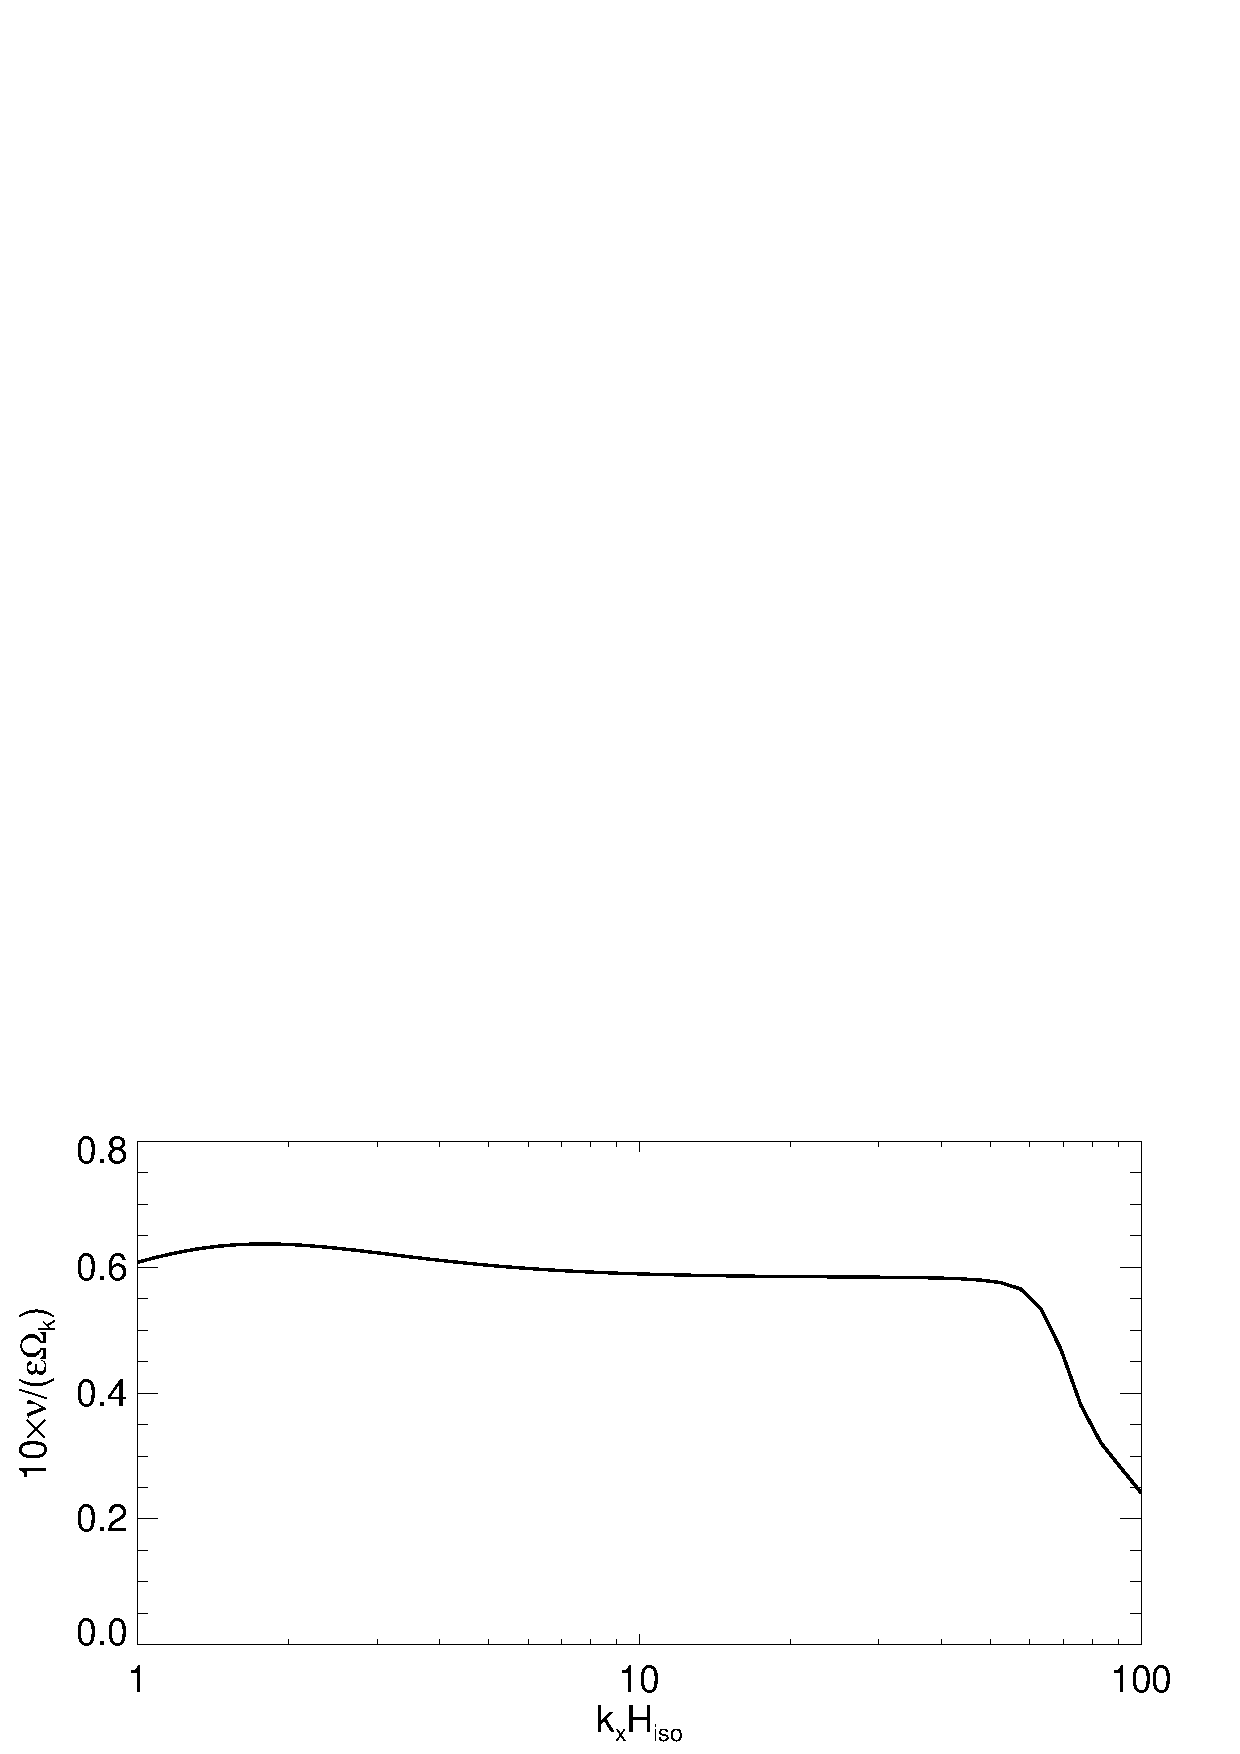
\includegraphics[width=\linewidth,clip=true,trim=0cm 0cm 0cm
  0cm]{figures/growth_mmsn_50AU} 
  \caption{VSI growth rates in the MMSN at
    $r=50\mathrm{AU}$. The thermal relaxation timescale $\beta(\khat)$
    used for this calculation is given by
    Eq. \ref{beta_mmsn} and is scale-dependent. 
    \label{mmsn_growth}}  
\end{figure}

% Fig. \ref{mmsn_eigenW} show several eigenfunctions for the modes in
% Fig. \ref{mmsn_growth}. As $\khat$ is increased, the disturbance
% become more concentrated near the vertical boundaries. Thus, modes
% with very large $\khat$ may not be important in practice because they
% predominantly affect the disk atmosphere, which contains little mass.  

\begin{figure}
   \includegraphics[width=\linewidth,clip=true,trim=0cm 0.0cm 0cm
  0cm]{figures/eigenvectorW_mmsnkx30.ps}
  % \includegraphics[width=\linewidth,clip=true,trim=0cm 1.75cm 0cm
  % 0cm]{figures/eigenvectorW_mmsnkx10.ps} 
  % \includegraphics[width=\linewidth,clip=true,trim=0cm 0cm 0cm
  % 0cm]{figures/eigenvectorW_mmsnkx50.ps} 
  \caption{Fundamental VSI mode in the MMSN at 
    $r=50\mathrm{AU}$. The eigenfunction $W$ for $\khat=30$ is shown. The real (imaginary)
    part of $W$ is plotted as the solid (dotted)
    lines. The thermal relaxation timescale $\beta(\khat)$ is given by
    Eq. \ref{beta_mmsn} and is scale-dependent. \label{mmsn_eigenW}}    
\end{figure}
% only find one unstable mode -> close to marginal 
% larger kx 

\subsubsection{Vertically-depedent thermal relaxation} 
Note that for a vertically isothermal disk and opacity $\kappa_d(T)$, 
we can restore the $z$ dependence in $\beta$ (due to the $\rho$
dependence in  $\eta$, see Eq. \ref{eta_def}) by making the transformation
$\beta(\khat)\to\beta(\khat/\sqrt{2\pi}\hat{\rho})\equiv 
\tilde{\beta}(\khat,z)$ in  Eq. \ref{real_beta}, where
$\hat{\rho}=\rho/\rho(z=0)$.  We have repeated the example
calculation above with $\beta\to\tilde{\beta}$, but found similar
results. 
%We find growth rates
%were reduced, but at most by $\sim 15\%$ at $\khat=1$. Eigenfunctions
%were similar.  


%at most by 15%
